\chapter{Literature Review}
\label{chap:literature_review}
The literature review presented in this chapter focuses specifically on the topic of custom loss functions, which is directly aligned with the primary focus of this thesis.  More specifically, this chapter provides a comprehensive overview of some of the most recent publications in this area, focusing on studies that, like this one, advocate for the use of loss function combinations or loss adjustments, to create a more precise learning signal than what standard loss functions can offer. While there is a wide range of literature available on loss functions and strategies for their enhancement, to the best of the authors' knowledge, no unified framework exists that systematically combines a predetermined set of prominent loss types in the manner suggested in this work.

For a more general review of semantic segmentation improvement strategies beyond the scope of this thesis, please refer to Appendix D: \squote{\nameref{chap:extended_literature_review}}.

\squote{Relax and focus on brain tumor segmentation} \cite{WANG2022102259} from 2022, presents a \ac{CNN} for fully automatic brain tumor segmentation. The authors of the paper acknowledge that one of the major challenges to accurately segmenting brain tumors is the great variation in location, size, structure, and morphological appearance, as well as the severe data imbalance that exist between brain tumors and non-tumor tissue, as well as among the different sub-regions within the brain tumor itself.

To address these challenges, the authors propose a hybrid model which incorporates several key components:
\begin{itemize}
    \item A dynamic combination of the \ac{FL} and \ac{DL} specifically designed to focus more on the smaller tumor sub-regions with more complex structures during the training process.
    \item A relaxation of boundary constraints for the inner tumor regions in a coarse-to-fine fashion to better recognize the overall structure of the brain tumor and the morphological relationship among different tumor sub-regions.
    \item A symmetric attention branch highlights the possible location of the brain tumor from the asymmetric features caused by the growth and expansion of abnormal brain tissues.
\end{itemize}

The authors of the paper claim that the proposed hybrid model can balance the learning capacity of the model between spatial details and high-level morphological features and can improve the overall segmentation performance of brain tumors. The model is validated on the publicly available brain tumor dataset from real patients called BRATS  2019 \cite{Menze2014-gj}. The experimental results show that their model improves the overall segmentation performance compared to the top approaches in the BRATS 2019 challenge.

\squote{PolyLoss: A Polynomial Expansion Perspective of Classification Loss Functions} \cite{leng2022polyloss} from 2022, presents a new framework named PolyLoss whose goal is to understand better and design loss functions for \acp{DNN}. The authors propose that commonly used classification loss functions such as \ac{CE} and \ac{FL} can be decomposed into a series of weighted polynomial functions. This framework allows for the importance of different polynomial bases to be adjusted depending on the target task and dataset. It demonstrates that better results can be achieved by adjusting these weights than with the commonly used loss functions. They also propose a simple and effective Poly-1 loss formulation that outperforms \ac{CE} and \ac{FL} on various tasks by only introducing one extra hyperparameter and adding one line of code.

\squote{Distribution-Aware Margin Calibration for Semantic Segmentation in Images} \cite{Yu2022} from 2022, describes a method to improve the performance of semantic segmentation models. The authors propose using a \squote{margin calibration} method, which can be used as a learning objective to improve the generalization of the IoU metric over the data distribution. The method theoretically ensures better segmentation performance in terms of \ac{IoU}. It has been evaluated on seven image datasets, showing substantial improvements in the IoU score over other learning objectives using deep segmentation models. In contrast, traditional loss functions, such as \ac{CE}, tend to have a poor indicator of model quality in semantic segmentation because the minimization of it does not guarantee a higher IoU score, which is more commonly used in semantic segmentation, specifically for sketching the contours of interest regions.

\squote{blob loss: instance imbalance aware loss functions for semantic segmentation} \cite{https://doi.org/10.48550/arxiv.2205.08209} from 2022, presents a new loss function called \squote{blob loss} for semantic segmentation tasks, which aims to improve instance-level detection metrics, such as F1 score and sensitivity.\footnote{$F1=\frac{2\cdot \text{Precision}\cdot \text{Recall}}{\text{Precision}+\text{Recall}}$} The authors argue that traditional loss functions, such as the \ac{DL}, do not take instance imbalance\footnote{Instance imbalance within a class occurs when there is a disproportionate number of instances with specific characteristics compared to others. Characteristics in this context could be different textures or morphological differences like size or shape \cite{https://doi.org/10.48550/arxiv.2205.08209}. For example, in a forest image dataset, there might be many trees with leaves but only a few without. Similarly, there could be significant and small tumors of the same class in medical imaging. This imbalance can lead to poor overall performance as models may struggle to identify less common instances accurately.} within a class into account, which can lead to sub-optimal results when the object of interest is highly heterogeneous. This is particularly relevant in medical applications, such as disease progression monitoring, where detecting small-scale lesions is critical. The proposed method is based on converting any loss function into a \squote{blob loss} by adding a term that represents the instance imbalance. This term is calculated as the ratio of the number of pixels belonging to the smaller instances to the number of pixels belonging to the more significant instances. The \squote{blob loss} is designed to work with semantic segmentation problems where the instances are connected components within a class.

The proposed method is evaluated on five complex 3D semantic segmentation tasks that feature pronounced instance heterogeneity in terms of texture and morphology. These tasks include multiple sclerosis lesions, liver tumors, and microscopy segmentation. The evaluation results showed that compared to the traditional soft \ac{DL}, the \squote{blob loss} achieved an average 2\% improvement for microscopy segmentation tasks considering F1 score and 5\% improvement for MS lesions.

The paper argues that the proposed \squote{blob loss} method addresses the issue of instance imbalance in semantic segmentation tasks, which is not adequately reflected in traditional loss functions such as \ac{DL}, and it can improve the performance of the model in detecting small scale lesions in medical applications.

\squote{Topology-Aware Segmentation Using Discrete Morse Theory} \cite{hu2021topologyaware} from 2021 proposes a new loss function incorporating topological information from the image segmentation task. The loss function is based on the concept of \ac{DMT}, a mathematical framework that uses the gradient vector field of the likelihood function to identify critical points and structures in the image. These structures, composed of 1D and 2D manifold pieces, reveal the topological information captured by the likelihood function. For more detailed information on \ac{DMT}, see \figref{morse_theory}.

\begin{figure}[H]%[htbp]
    \centering
    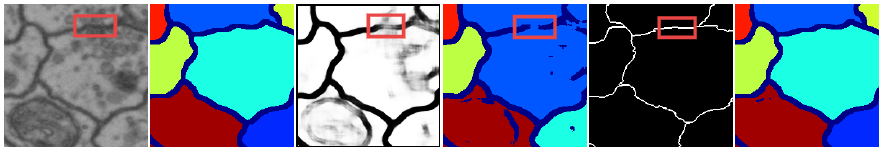
\includegraphics[width=\imgWidthXL]{images/morse_theory.png}
    \caption[\acf{DMT} predictions]{From left to right: Sample, Ground truth, Likelihood map, Baseline prediction, Critical structure with \ac{DMT} loss applied and final result. Image from \cite{hu2021topologyaware}}
    \label{morse_theory}
\end{figure}

The method identifies these critical structures, called Morse structures, as essential for topological accuracy. The loss function assigns a higher penalty to predictions that deviate from these structures. This way, the network is encouraged to produce predictions more consistent with the topological information.

The loss function is designed to correct false negatives, where a structure is a tree structure missed in the segmentation, and false positives, where a structure is a \squote{halluzination} of the model and should be removed. By enforcing higher penalties along the identified Morse structures, the network is forced to predict correctly near these topologically difficult locations and address the sampling bias issue \footnote{Sampling bias is a problem that occurs when the sample used in a study or survey is not representative of the population being studied, leading to inaccurate or misleading results \cite{10.1145/3457607}.}.

In summary, the new loss function proposed in the paper uses the concept of discrete Morse theory to identify global structures and critical points in the image. It incorporates this topological information into the training process by assigning a higher penalty to predictions that deviate from these structures. This approach improves the network's performance, especially near topologically challenging locations, and ensures that the network can produce segmentations with correct topology.

\squote{Tilted Cross Entropy {(TCE):} Promoting Fairness in Semantic Segmentation} \cite{DBLP:journals/corr/abs-2103-14051} from 2021, proposes a new loss function called \ac{TCE} for semantic segmentation in order to minimize performance disparities among target classes and promote fairness. The \ac{TCE} is inspired by the recently introduced \ac{TERM}\cite{li2020tilted} and is adapted to the semantic segmentation setting. The authors demonstrate through quantitative and qualitative performance analyses that the proposed \ac{TCE} can improve the low-performing classes of CityScapes \cite{cordts2016cityscapes} and ADE20k \cite{zhou2017scene} datasets and also results in improved overall fairness.

\squote{Rethinking the Dice Loss for Deep Learning Lesion Segmentation in Medical Images} \cite{9338261} from 2021 presents four limitations called \emph{Distance insensitivity}, \emph{Boundary insensitivity}, \emph{Region-size sensitivity} and \emph{Insensitivity to FP / FN weight}, for the \ac{DL} and how to overcome them. This section provides a detailed review of these limitations.

One significant weakness is the \squote{insensitivity to the distance} between non-overlapping regions, as highlighted by \cite{9338261}. This means that regardless of how far these regions are apart, the loss will remain constant even if, intuitively, a closer region should yield a lower loss. A computational example using the \ac{DL} is illustrated in \figref{dice_limit_1}.
\begin{figure}[H]%[htbp]
  \centering
  \subfigure[]{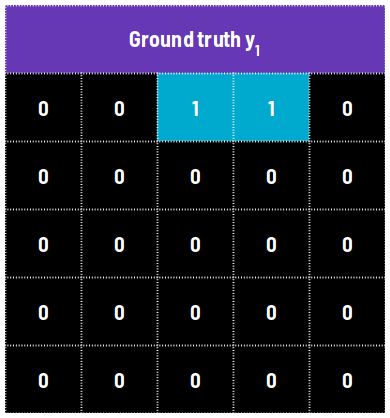
\includegraphics[width=\imgWidthFour]{images/dice_limit_1_1.png}}
  \subfigure[]{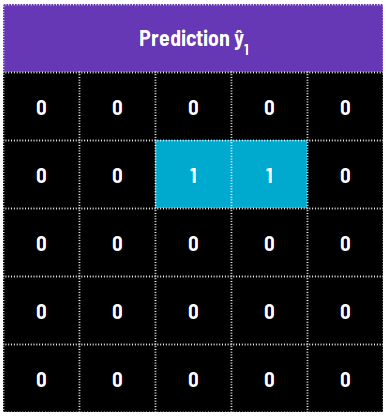
\includegraphics[width=\imgWidthFour]{images/dice_limit_1_2.png}}
  \subfigure[]{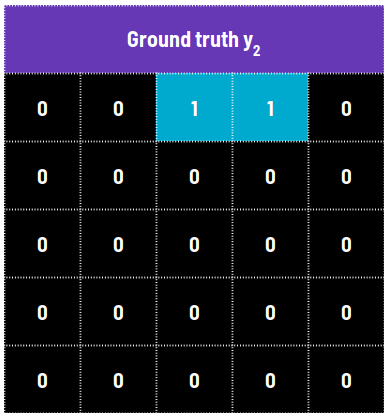
\includegraphics[width=\imgWidthFour]{images/dice_limit_1_3.png}}
  \subfigure[]{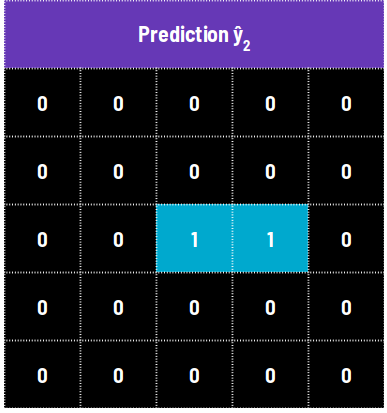
\includegraphics[width=\imgWidthFour]{images/dice_limit_1_4.png}}
  \caption[Distance insensitivity of \ac{DL}]{The images show the insensitivity to distance of the \ac{DL}. Image (a) and (c) depict the ground truths $y_1,y_2$, and image (b) and (d) the corresponding predictions $\hat{y}_1,\hat{y}_2$. It can be seen that even if $\hat{y}_1$ is closer to the ground truth than $\hat{y}_2$ the result for both predictions is the same with $DL_1=DL_2=1-\frac{2\cdot 0}{2\cdot 0 + 2 + 2}=1.0$.}
  \label{dice_limit_1}
\end{figure}
An additional limitation of the \ac{DL} is its \squote{insensitivity to boundaries}. The loss function cannot accurately account for the precise contours of segmented regions and fails to reflect how the overlap occurs if the number of true positives stays the same. See \figref{dice_limit_2} for a detailed illustration of the issue.
\begin{figure}[H]%[htbp]
  \centering
  \subfigure[]{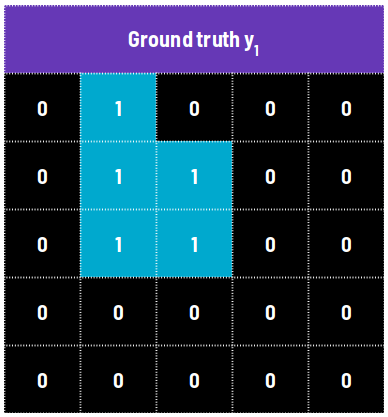
\includegraphics[width=\imgWidthFour]{images/dice_limit_2_1.png}}
  \subfigure[]{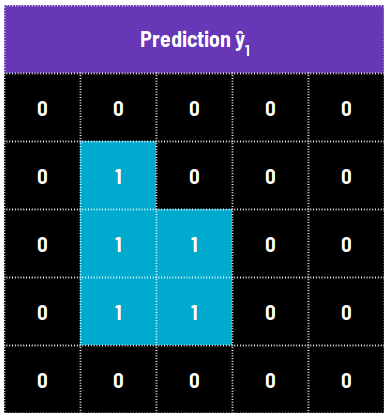
\includegraphics[width=\imgWidthFour]{images/dice_limit_2_2.png}}
  \subfigure[]{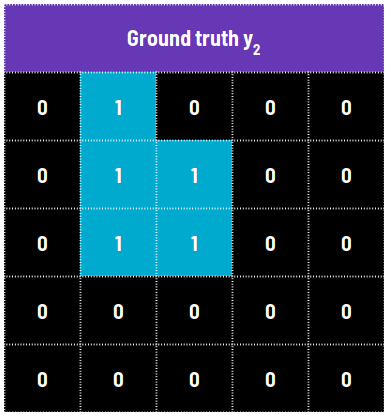
\includegraphics[width=\imgWidthFour]{images/dice_limit_2_3.png}}
  \subfigure[]{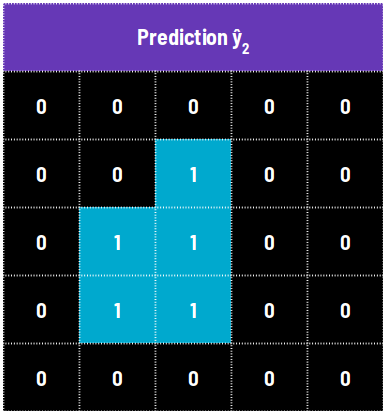
\includegraphics[width=\imgWidthFour]{images/dice_limit_2_4.png}}
  \caption[Boundary insensitivity of \ac{DL}]{The images demonstrate the boundary insensitivity of the \ac{DL}. Image (a) and (c) depict the ground truths $y_1,y_2$, and image (b) and (d) the corresponding predictions $\hat{y}_1,\hat{y}_2$. Despite their visual differences, both overlaps yield an identical loss with $DL_1=DL_2=1-\frac{2\cdot 3}{2\cdot 3 + 2 + 3}= 0.5$.}
  \label{dice_limit_2}
\end{figure}
Another notable limitation of the \ac{DL} is its \squote{sensitivity to region size}. Consider a scenario where a large region needs to be predicted. If a single pixel is misclassified, the resulting loss is much lower than if a pixel is misclassified when predicting smaller regions. See \figref{dice_limit_3} for further illustration.
\begin{figure}[H]%[htbp]
  \centering
  \subfigure[]{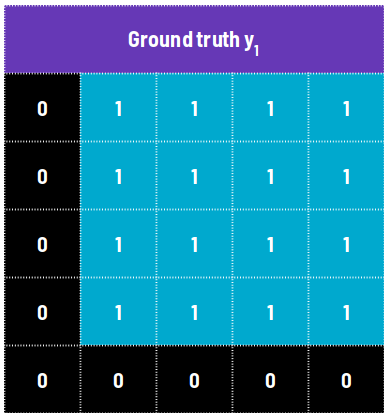
\includegraphics[width=\imgWidthFour]{images/dice_limit_3_1.png}}
  \subfigure[]{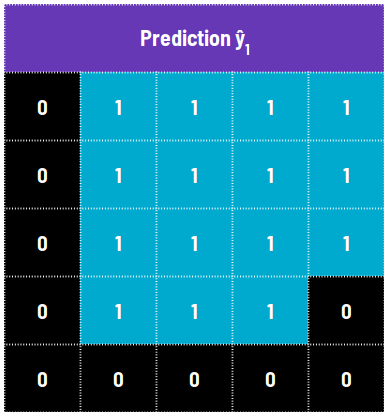
\includegraphics[width=\imgWidthFour]{images/dice_limit_3_2.png}}
  \subfigure[]{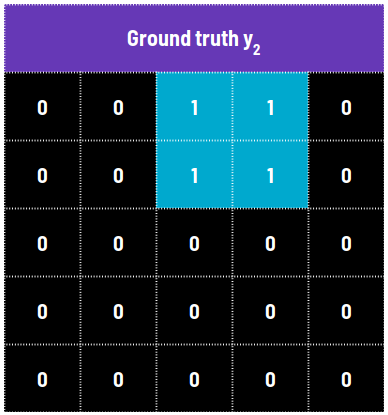
\includegraphics[width=\imgWidthFour]{images/dice_limit_3_3.png}}
  \subfigure[]{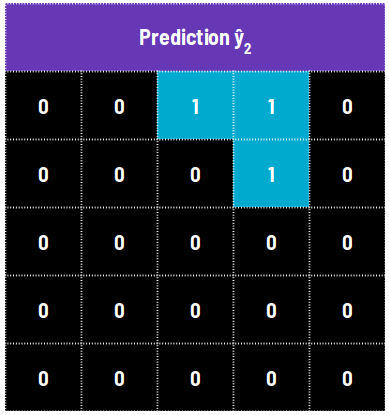
\includegraphics[width=\imgWidthFour]{images/dice_limit_3_4.png}}
  \caption[Sensitivity towards small region of \ac{DL}]{The images demonstrate the sensitivity towards small regions. In images (a) and (b), the ground truth $y$ and prediction $\hat{y}$ have a misclassification of one pixel, resulting in a \ac{DL} of $DL_1=1-\frac{2\cdot 15}{2\cdot 15 + 0 + 1}\approx 0.03$. On the other hand, in the image (c) and (d), the misclassification occurs on a smaller region resulting in a higher \ac{DL} of $DL_2=1-\frac{2\cdot 3}{2\cdot 3 + 0 + 1}\approx 0.142$}
  \label{dice_limit_3}
\end{figure}
A further limitation of the \ac{DL}, described in \cite{9338261}, is its \squote{insensitivity to FP / FN weight}, or which can be a disadvantage since, depending on the task, researchers want to weigh false positives or false negatives differently. To illustrate this limitation, consider the example shown in \figref{dice_limit_4}.
\begin{figure}[H]%[htbp]
  \centering
  \subfigure[]{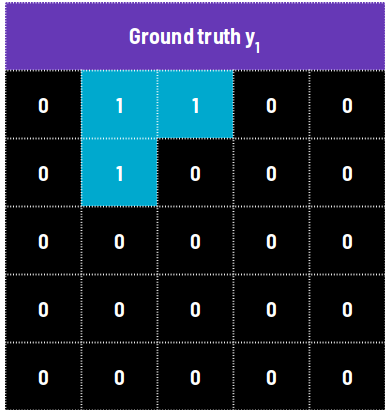
\includegraphics[width=\imgWidthFour]{images/dice_limit_4_1.png}}
  \subfigure[]{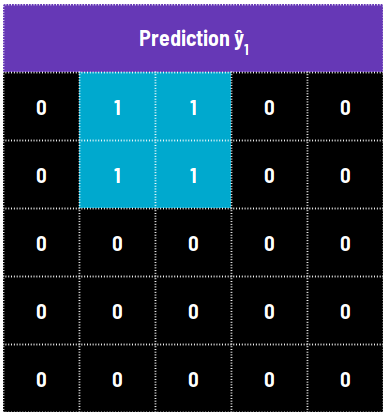
\includegraphics[width=\imgWidthFour]{images/dice_limit_4_2.png}}
  \subfigure[]{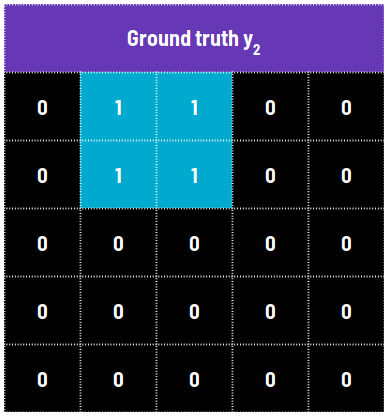
\includegraphics[width=\imgWidthFour]{images/dice_limit_4_3.png}}
  \subfigure[]{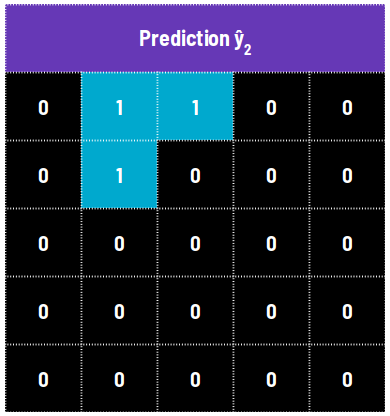
\includegraphics[width=\imgWidthFour]{images/dice_limit_4_4.png}}
  \caption[Insensitivity to FP / FN weight \ac{DL}]{The concept of insensitivity to the weight put on false negative and false positive predictions is demonstrated in this figure. The loss from (a) and (b) $DL_1 = 1-\frac{2*3}{2*3+1+0}\approx 0.142$ is the same as the loss from (c) and (d) $DL_2 = 1-\frac{2*3}{2*3+0+1}\approx 0.142$.}
  \label{dice_limit_4}
\end{figure}

\newpage